\documentclass[border=10pt]{standalone}
\usepackage[svgnames]{xcolor}
\usepackage{amsmath}
\usepackage{pgfplots}
\pgfplotsset{compat=newest}
\usepackage[sfdefault]{FiraSans}
\usepackage{FiraMono}
\renewcommand*\familydefault{\sfdefault}
\begin{document}
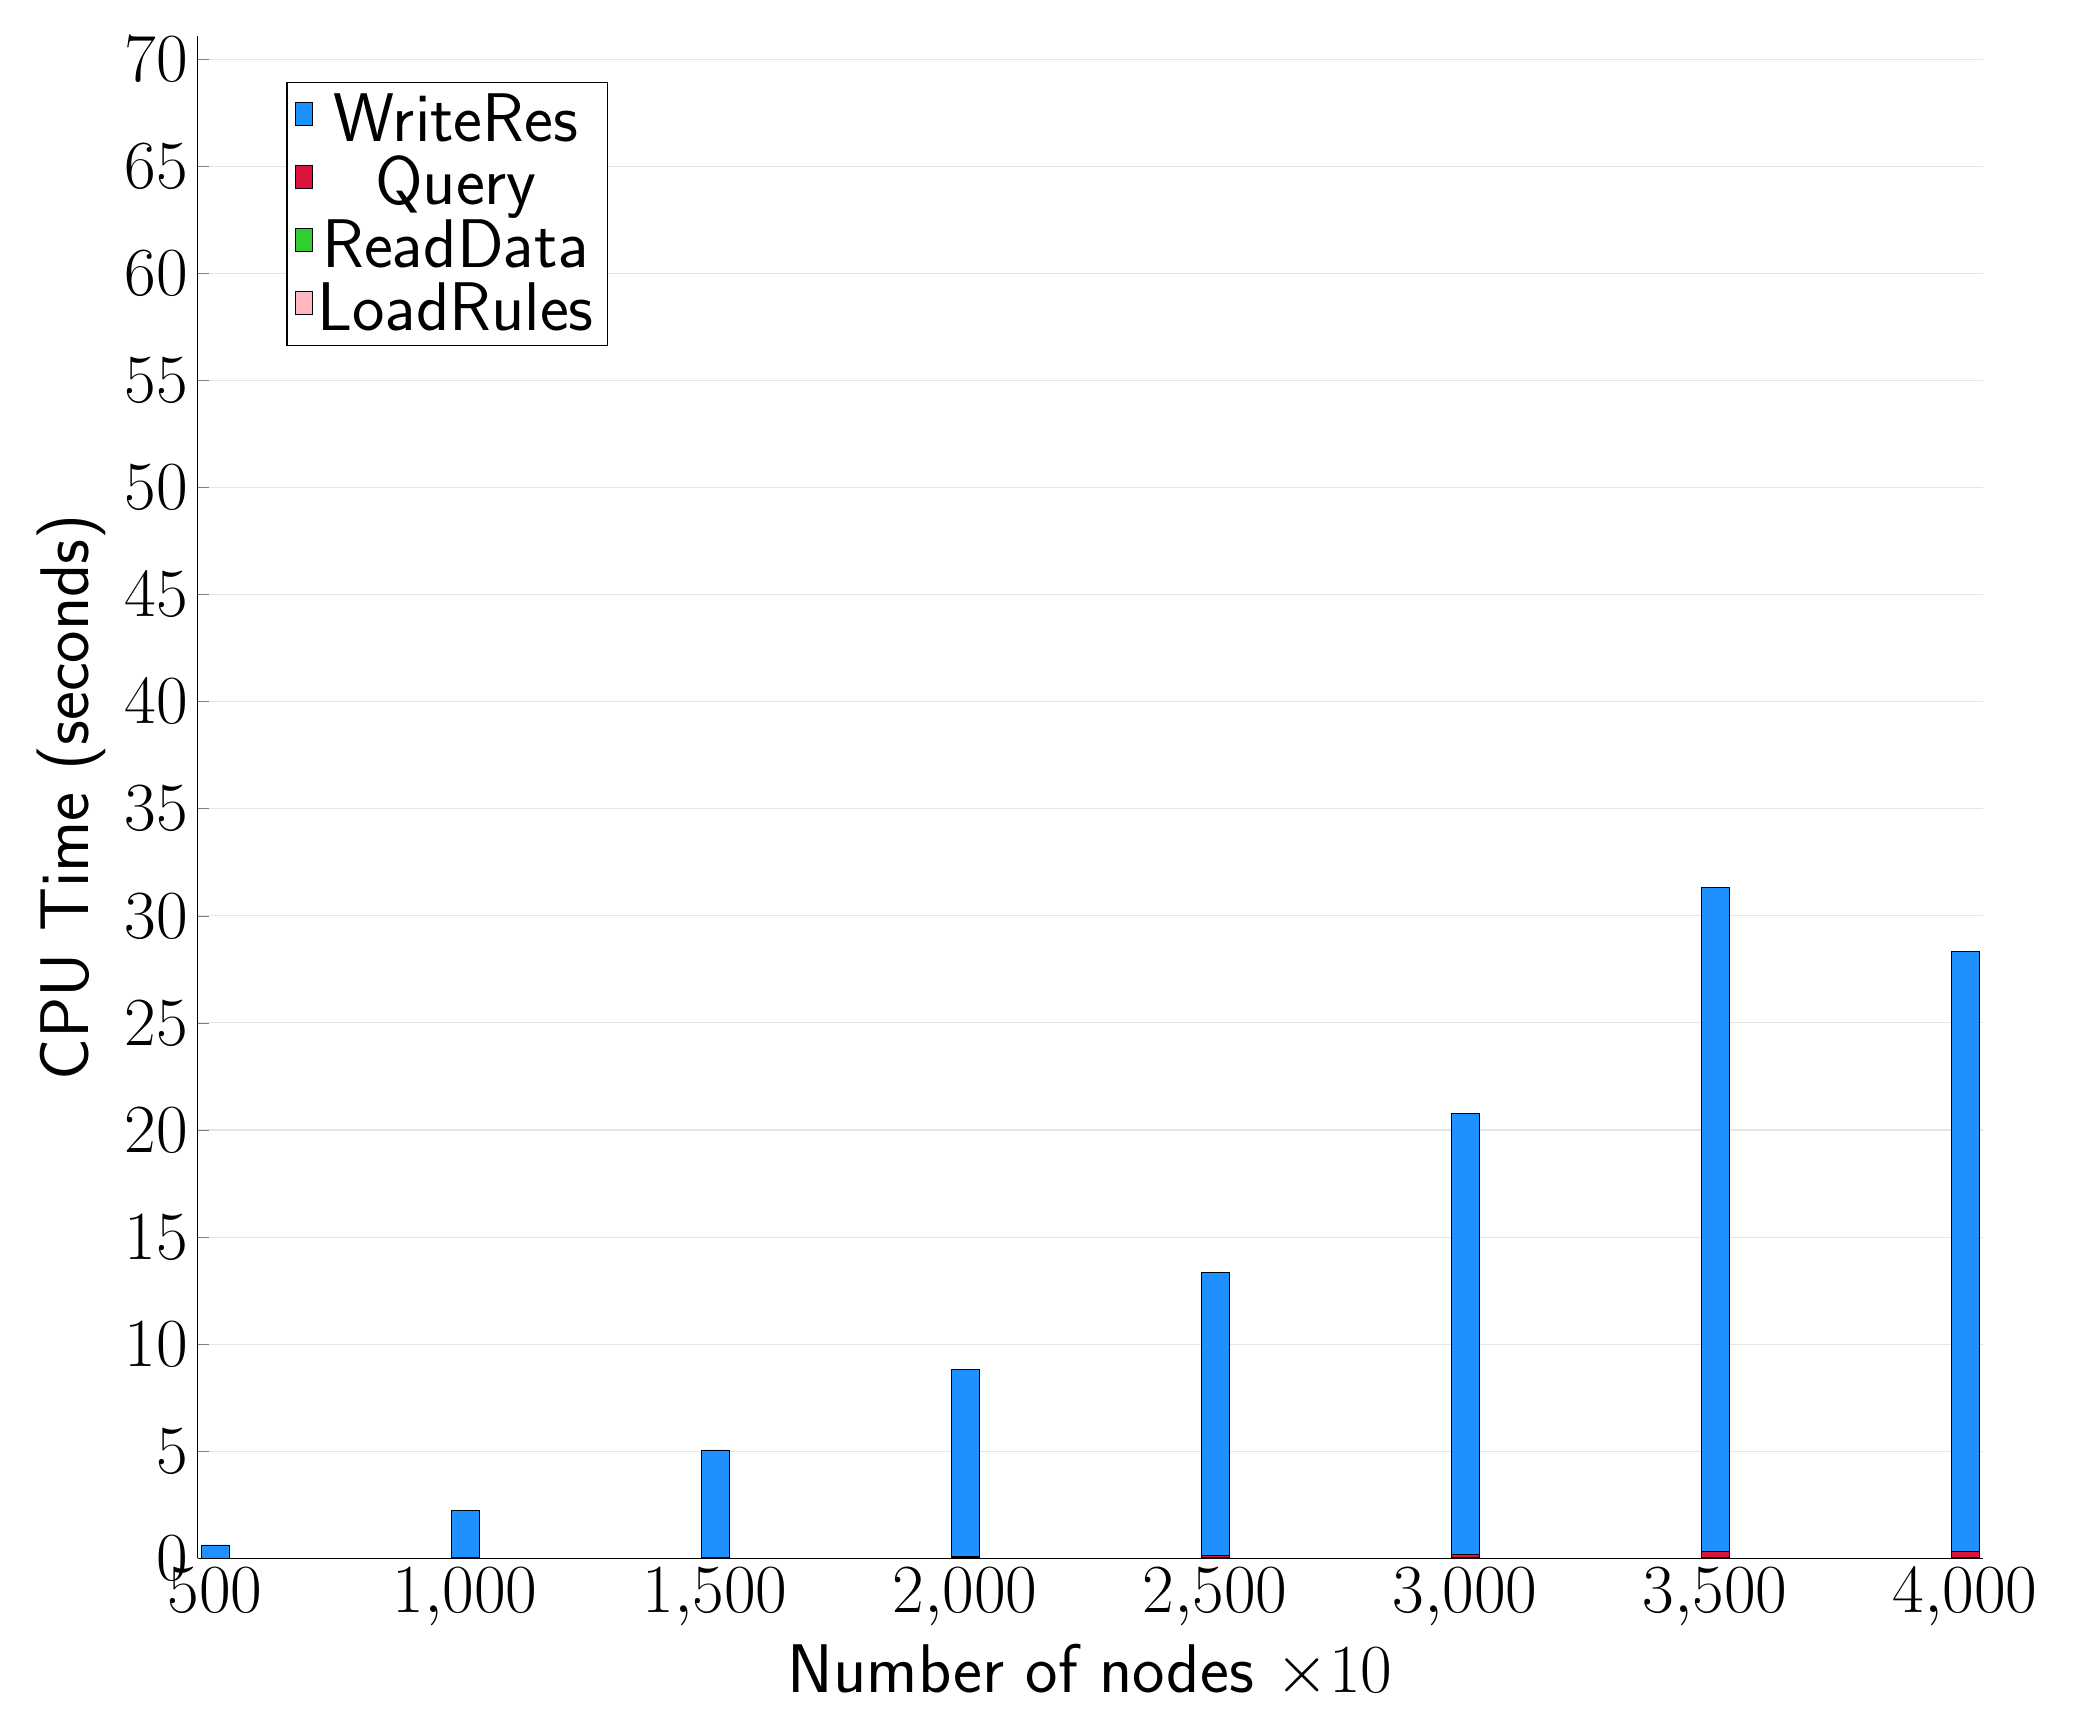
\begin{tikzpicture}
\begin{axis}[
   ybar stacked,
   width=2\textwidth,
   bar width=0.35cm,
   ymajorgrids, tick align=inside,
   major grid style={draw=gray!20},
   xtick=data,
   ymin=0, ymax=71.079008658727,
   axis x line*=bottom,
   axis y line*=left,
   enlarge x limits=0.01,
   legend style={
       at={(0.23, 0.97)},
       anchor=north east,
       legend columns=1,
       font=\Huge,
   },
   ylabel={CPU Time (seconds)},
   xlabel={Number of nodes $\times 10$},
   label style={font=\Huge},
   tick label style={font=\Huge},
]
\addlegendimage{fill=DodgerBlue, draw=black, line width=0.2pt}
\addlegendentry{WriteRes}
\addlegendimage{fill=Crimson, draw=black, line width=0.2pt}
\addlegendentry{Query}
\addlegendimage{fill=LimeGreen, draw=black, line width=0.2pt}
\addlegendentry{ReadData}
\addlegendimage{fill=LightPink, draw=black, line width=0.2pt}
\addlegendentry{LoadRules}
\addplot +[fill=LightPink, draw=black, line width=0.2pt] coordinates {
(500, 0.0049440000000000005)
(1000, 0.004467666666666673)
(1500, 0.0033053333333333303)
(2000, 0.004451666666666664)
(2500, 0.004563)
(3000, 0.0044863333333333335)
(3500, 0.004998333333333337)
(4000, 0.0037359999999999997)
};
\addplot +[fill=LimeGreen, draw=black, line width=0.2pt] coordinates {
(500, 0.010025999999999998)
(1000, 0.015916666666666666)
(1500, 0.023359)
(2000, 0.029436)
(2500, 0.03692566666666667)
(3000, 0.04203833333333334)
(3500, 0.055746)
(4000, 0.04949633333333334)
};
\addplot +[fill=Crimson, draw=black, line width=0.2pt] coordinates {
(500, 0.003293333333333337)
(1000, 0.014888666666666666)
(1500, 0.03638333333333333)
(2000, 0.07140866666666668)
(2500, 0.11055366666666666)
(3000, 0.1566753333333333)
(3500, 0.25434066666666666)
(4000, 0.261251)
};
\addplot +[fill=DodgerBlue, draw=black, line width=0.2pt] coordinates {
(500, 0.6094946666666666)
(1000, 2.214624)
(1500, 5.005539)
(2000, 8.701642000000001)
(2500, 13.194564666666666)
(3000, 20.590858333333333)
(3500, 31.00154466666667)
(4000, 28.023601)
};
\end{axis}
\end{tikzpicture}

\end{document}
